%!TEX TS-program = xelatex
\documentclass[aspectratio=169]{beamer}
\usetheme{hust}

\usepackage{graphicx}
\usepackage{tikz}
\usepackage{calc}
\usepackage{polyglossia}
\setmainlanguage{english}
\usepackage{amsthm,amsmath,amssymb}
\newtheorem{thm}{Theory}
\newtheorem{defn}{Definition}
\usepackage{subcaption}
\usepackage{dutchcal}
\usepackage[authoryear, comma, sort&compress]{natbib}

\setbeameroption{show notes} % show notes and slides
% \setbeameroption{hide notes} % Only slides
% \setbeameroption{show only notes} % show only notes
\addtobeamertemplate{note page}{}{\thispdfpagelabel{notes:\insertframenumber}}
\setbeamertemplate{note page}[plain]
\setbeamertemplate{theorems}[numbered]
\setbeamertemplate{caption}[numbered]

\newcommand{\Image}[1]{%
    \sbox0{\includegraphics[height=0.65\paperheight]{#1}}%
    \ifdim\wd0 < \textwidth
    \includegraphics[height=0.65\paperheight]{#1}%
  \else
  \includegraphics[width=\textwidth]{#1}%
  \fi%
}

\newif\iffirsttoc
\firsttoctrue
\AtBeginSubsection[]
{
    \begin{frame}
        \frametitle{Table of contents}
        \iffirsttoc
            \tableofcontents
            \global\firsttocfalse
        \else
            \tableofcontents[currentsection,
            % hideothersubsections,
            subsectionstyle=show/shaded/hide,
            subsubsectionstyle=show/show/show/hide
            ]
        \fi
    \end{frame}
}

% \titlegraphic{\includegraphics[height=\logoheight]{figures/sami-v2.pdf}}
\title{Graduation Thesis}
\subtitle{Grammatical Error Correction Using Machine Learning\\Web Application}

\author{Student: Ngô Văn Cảnh - 20193204 \protect\linebreak Advisor: Prof. Dương Tấn Nghĩa}

\date{February 2025}

\begin{document}
\begin{frame}[noframenumbering,Title]
  \maketitle
\end{frame}

\note{
  Greatings, everyone.
  I am Ngô Văn Cảnh from Hanoi University of Science and Technology. % TODO: this is a bit redundant, maybe remove it
  Today, I am going to present my graduation thesis, which is about Grammatical Error Correction Using Machine Learning Web Application.
  My advisor is Professor Dương Tấn Nghĩa. %TODO: does it need to be mentioned here?
}

\section{Introduction}

\subsection{Motivation}

\begin{frame}{Motivation}
  \begin{figure}
    \begin{center}
      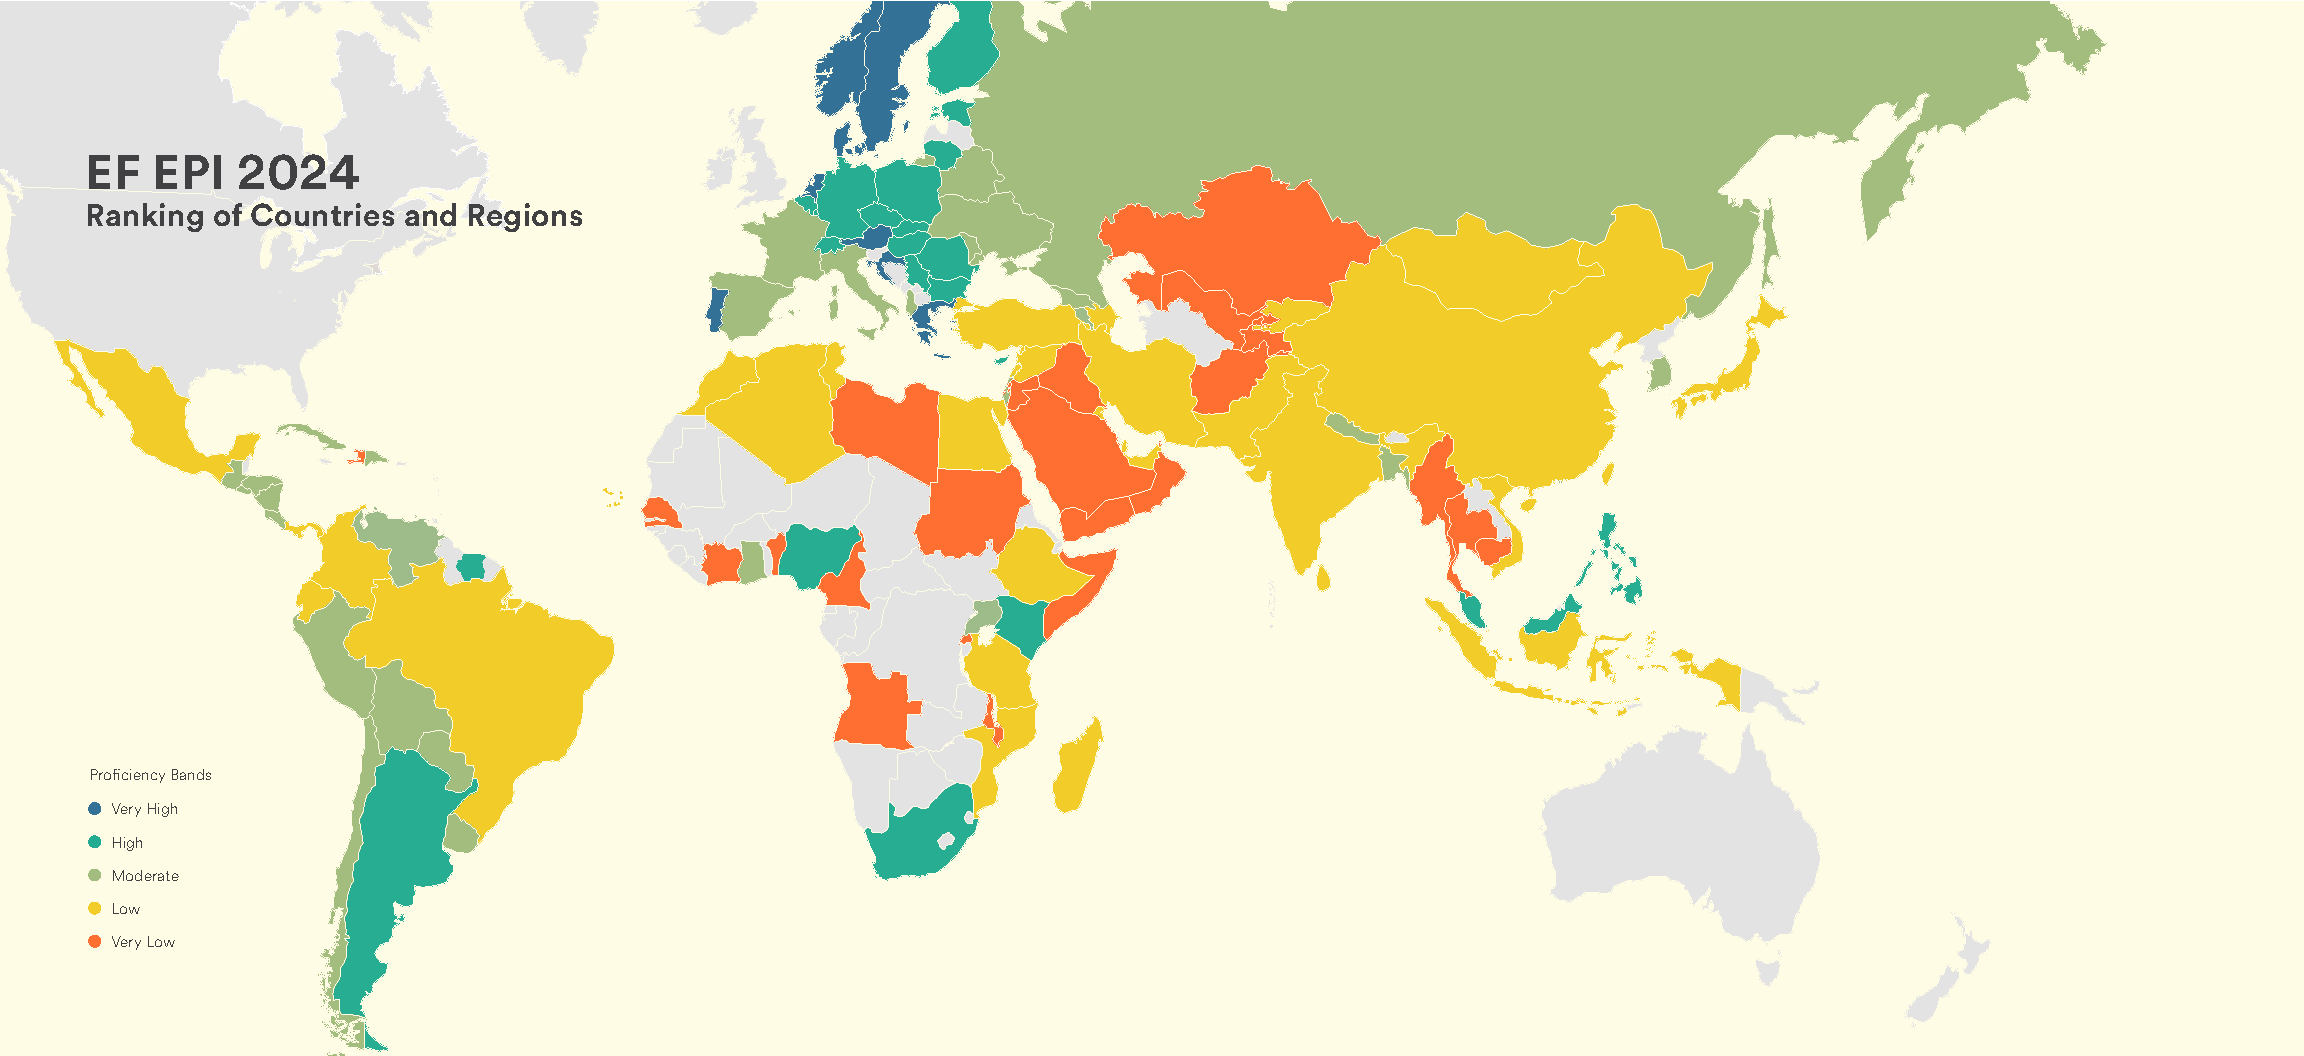
\includegraphics[width=\textwidth]{figures/ef-epi-2024-english-crop.pdf}
      \begin{textblock*}{8cm}(\paperwidth-9cm, \paperheight-2.5cm)  % (x,y) coordinates from top-left
        \textbf{\Large $> 1.4$ billion speakers}

        \textbf{\Large $\sim 75\%$ non-native}
      \end{textblock*}
    \end{center}
    \caption{English Proficiency bands by countries \citeyear{ef-epi-2024}}\label{fig:ef-epi}
  \end{figure}
\end{frame}

\note{
  English is one of the most widely used languages globally,
  spoken by approximately more than 1.4 billion speakers, with almost 75\% of them being non-native speakers
  As the number of esl and efl learners continues to grow, the need for effective language learning tools and resources has increased significantly.
  However, grammatical and spelling errors remain common challenges for many writers, affecting clarity and professionalism.
}

% \begin{frame}{Motivation}
%   English is one of the most widely used languages globally, serving as a common medium of communication for over \alert{1.4 billion} people worldwide, with almost \alert{75\%} of them being non-native speakers~\citep{eberhard2015ethnologue}.
%   As the number of esl and efl learners continues to grow, the demand for effective language learning tools and resources has increased significantly.
%   However, grammatical and spelling errors remain common challenges for many writers, affecting clarity and professionalism.
% \end{frame}

\subsection{Definition of Grammatical Error Correction (GEC)}

\begin{frame}{Definition of Grammatical Error Correction}
  \centering
  {\Huge
    \textcolor{red}{G}rammatical
    \textcolor{red}{E}rror
    \textcolor{red}{C}orrection
  }

  \vfill

  {\Large
    He \textcolor{red}{go} to the store and \textcolor{red}{buyed} some \textcolor{red}{apple's}.
  }

  \noindent\rule[0.5ex]{\linewidth}{1pt}

  {\Large
    He \textcolor{green}{goes} to the store and \textcolor{green}{bought} some \textcolor{green}{apples}.
  }

  \vfill
\end{frame}

\note{
  Grammatical Error Correction is the task of automatically detecting and correcting errors in text.
  The task not only includes the correction of grammatical errors, such as missing prepositions and mismatched subject-verb agreement but also orthographic and semantic errors, such as misspellings and word choice errors.
  The term Grammatical Error Correction is thus something of a misnomer but is nevertheless now commonly understood to encompass errors that are not always strictly grammatical in nature.
  A more descriptive term is Language Error Correction.
}

\section{Methodology}

\section{Implementation}

\section{Conclusion}


\section{References}
\begin{frame}{References}
  % \nocite{*}
  \bibliographystyle{plainnat}
  \bibliography{cite}
\end{frame}

\begin{frame}{~}
  \begin{center}
    \Large \color{hustred}{Thank you for your attention!}
  \end{center}
\end{frame}

\end{document}
